% id: 41-07
% book: 베이직쎈 확률과 통계 · 03 확률의 뜻과 활용
% section: 유형 023 배반사건
% figure: tikz:fig-41-07
% answer: 
% answer_source: 
% variant_level: 0 (원본 전사)
% 이 파일은 build.mjs 가 items.json 에서 만든다. 고칠 때는 items.json 을 고친다.
\smash{\raisebox{1.5mm}{\dmkichul{베이직쎈 확률과 통계 41쪽 07번}}}
\noindent\begin{minipage}[t]{0.58\linewidth}\vspace{0pt}\raggedright 오른쪽 그림과 같은 전개도로 만든 정육면체를 던지는 시행에서 바닥에 닿는 면에 적힌 수가 2의 배수인 사건을 $A$, 3의 배수인 사건을 $B$라 할 때, 다음 중 옳지 \underline{않은} 것은?\end{minipage}\hfill\begin{minipage}[t]{0.4\linewidth}\vspace{0pt}\centering \resizebox{\ifdim\width>\linewidth\linewidth\else\width\fi}{!}{% 유형 023 41-07(인쇄 41쪽) — 정육면체의 전개도(십자 모양). 가운데 세로줄 1·2·9·8, 가운데 칸 2의 양옆에 3·7.
%   스캔 화질이 낮아 TikZ 로 다시 그림. 바깥 테두리는 실선, 접는 선은 원문대로 점선.
% 라벨은 원문에 있는 숫자만 넣는다(답은 그림에서 읽히지 않는다 — 전개도의 수는 문제의 주어진 조건).
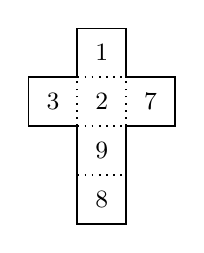
\begin{tikzpicture}[scale=0.62, line width=0.5pt]
  % 바깥 테두리
  \draw[line width=0.6pt] (1,4) -- (2,4) -- (2,3) -- (3,3) -- (3,2) -- (2,2) -- (2,0) -- (1,0) -- (1,2) -- (0,2) -- (0,3) -- (1,3) -- cycle;
  % 접는 선(원문의 점선)
  \draw[dotted, line width=0.6pt] (1,3) -- (2,3);
  \draw[dotted, line width=0.6pt] (1,2) -- (2,2);
  \draw[dotted, line width=0.6pt] (1,1) -- (2,1);
  \draw[dotted, line width=0.6pt] (1,2) -- (1,3);
  \draw[dotted, line width=0.6pt] (2,2) -- (2,3);
  \node[font=\small] at (1.5,3.5) {$1$};
  \node[font=\small] at (0.5,2.5) {$3$};
  \node[font=\small] at (1.5,2.5) {$2$};
  \node[font=\small] at (2.5,2.5) {$7$};
  \node[font=\small] at (1.5,1.5) {$9$};
  \node[font=\small] at (1.5,0.5) {$8$};
\end{tikzpicture}
}\end{minipage}\par
\par\medskip\par\noindent\hangindent=1.4em\hangafter=1 {\small ①}\ $A=\{2{,}\mkern3mu\mathopen{}8\}$\par\noindent\hangindent=1.4em\hangafter=1 {\small ②}\ $B=\{3{,}\mkern3mu\mathopen{}9\}$\par\noindent\hangindent=1.4em\hangafter=1 {\small ③}\ $A\not\subset \comp{B}$\par\noindent\hangindent=1.4em\hangafter=1 {\small ④}\ 두 사건 $A$와 $B$는 서로 배반사건이다.\par\noindent\hangindent=1.4em\hangafter=1 {\small ⑤}\ 이 시행의 근원사건은 $\{1\}$, $\{2\}$, $\{3\}$, $\{7\}$, $\{8\}$, $\{9\}$이다.\par\medskip
